% !TEX spellcheck = en_US



% ~~~~~~~~~~~~~~~~~~~~~~~~~~~~~~~~~~~~~~~ V
% (NC) 2026 Haluk Bingol
% github.com/halukbingol/LaTeX-Templates
%
% Licensees may copy, distribute, display, and perform the work and make derivative works 
% and remixes based on it only for non-commercial purposes. 
% ~~~~~~~~~~~~~~~~~~~~~~~~~~~~~~~~~~~~~~~ A




% =====================================================================
%  Java on the Command Line -- Senior Level: Inside the Launcher, Security and Delivery
%  ---------------------------------------------------------------------
%  Built on hbCisLaTeXTemplate.tex with the libraries in ../../hblib/.
%  Programs, terminal sessions and their real outputs are in codeoutput/:
%     codeoutput/<Name>.java  a program        codeoutput/<Name>.sh   a session
%     codeoutput/<Name>/      the session's project folder
%     codeoutput/<Name>.txt   what it printed, made by:  bash run_examples.sh
% =====================================================================

\documentclass[aspectratio=169,10pt,compress]{beamer}

% ~~~~~~~~~~~~~~~~~~~~~~~~~~~~~~~~~~~~~~~~~~~~~~~~~~~~~~~~~~~~~~~~~ V hblib
	\usepackage{../../hblib/hblibPresentation} % lib presentation: theme, i/N, \hSection, algorithm2e, ...
	\usepackage{../../hblib/hblibCodeoutput} % lib code + output: \lstcode, \lstterminal, ...
	\usepackage{../../hblib/hblibDatastructures} % lib data structures: \hString, \hStack, \hQueue
% ~~~~~~~~~~~~~~~~~~~~~~~~~~~~~~~~~~~~~~~~~~~~~~~~~~~~~~~~~~~~~~~~~ A hblib


% xcolor, array (and the L{width} column), listings, tikz and algorithm2e come from the hblib libraries
\usepackage[T1]{fontenc}
\usepackage{lmodern}
\usepackage{booktabs}

\definecolor{gitred}{RGB}{240,80,50}
\newcommand{\win}{\textbf{Windows}}
\newcommand{\mac}{\textbf{macOS}}
\lstdefinelanguage{text}{}

% ---------------------------------------------------------------------
\title{Java on the Command Line}
\subtitle{Senior Level: Inside the Launcher, Security and Delivery}
\author[Bingol]{Haluk O. Bingol}

\institute[FCIS]{
    Faculty of Computer and Information Sciences\\
    Yeditepe University
}
\date{
	{\tiny \hbTimeStamp}
}

\begin{document}




% ~~~~~~~~~~~~~~~~~~~~~~~~~~~~~~~~~~~~~~ V frm
\begin{frame}[t,fragile]
  \titlepage
\end{frame}
% ~~~~~~~~~~~~~~~~~~~~~~~~~~~~~~~~~~~~~~ A frm




% ~~~~~~~~~~~~~~~~~~~~~~~~~~~~~~~~~~~~~~ V frm
\begin{frame}[t,fragile] \frametitle{Outline}
  \begin{columns}[T]
    \begin{column}{0.48\textwidth}
      \tableofcontents[sections={1-4}, hideallsubsections]
    \end{column}
    \begin{column}{0.48\textwidth}
      \tableofcontents[sections={5-8}, hideallsubsections]
    \end{column}
  \end{columns}
\end{frame}
% ~~~~~~~~~~~~~~~~~~~~~~~~~~~~~~~~~~~~~~ A frm

% ~~~~~~~~~~~~~~~~~~~~~~~~~~~~~~~~~~~~~~ V
\hSection[Launcher]{Inside the java Launcher}{}{}
% ~~~~~~~~~~~~~~~~~~~~~~~~~~~~~~~~~~~~~~ A

% ~~~~~~~~~~~~~~~~~~~~~~~~~~~~~~~~~~~~~~ V
\subsection[Steps]{From command to main}
% ~~~~~~~~~~~~~~~~~~~~~~~~~~~~~~~~~~~~~~ A




% ~~~~~~~~~~~~~~~~~~~~~~~~~~~~~~~~~~~~~~ V frm
\begin{frame}[t,fragile] \frametitle{What happens when you type \texttt{java -cp out App}}
% +++++++++++++++++++++++++++++++++++++++ V alg
%: -Alg. 
\begin{algorithm}[H]
  \caption{The \texttt{java} launcher (simplified)}
  \KwIn{command line $c$, environment $e$}
  insert $e[\texttt{JDK\_JAVA\_OPTIONS}]$ before the options of $c$; expand every \texttt{@file}\;
  split $c$ into JVM options, the main class (or \texttt{-jar} / \texttt{-m}) and the program arguments\;
  load the JVM library (\texttt{libjvm.so}, \texttt{jvm.dll}, \texttt{libjvm.dylib}) and create the JVM\;
  the JVM reads $e[\texttt{JAVA\_TOOL\_OPTIONS}]$, maps the CDS archive, resolves the boot modules\;
  \eIf{\texttt{-jar} $f$}{$\mathit{main} \gets$ \texttt{Main-Class} of $f$; class path $\gets f$ + its \texttt{Class-Path}}{
    $\mathit{main} \gets$ the given class}
  load $\mathit{main}$ with the \textbf{application class loader}; link, verify, initialize\;
  call \texttt{main(String[])} on a new thread \texttt{main}\;
  wait for all non-daemon threads; run shutdown hooks; \Return{exit status}\;
\end{algorithm}
% +++++++++++++++++++++++++++++++++++++++ A alg

\end{frame}
% ~~~~~~~~~~~~~~~~~~~~~~~~~~~~~~~~~~~~~~ A frm




% ~~~~~~~~~~~~~~~~~~~~~~~~~~~~~~~~~~~~~~ V frm
\begin{frame}[t,fragile] \frametitle{Where the JDK lives}
  \begin{columns}[T]
    \begin{column}{0.48\textwidth}
      \begin{block}{\win}


% +++++++++++++++++++++++++++++++++++++++ V lst
%: -Lst.
\begin{lstlisting}[style=codesnippet, language={}, basicstyle=\ttfamily\scriptsize]
where java
echo %JAVA_HOME%
dir "C:\Program Files\Eclipse Adoptium"
\end{lstlisting}
% +++++++++++++++++++++++++++++++++++++++ A lst


      \end{block}
      \small Installers add \texttt{bin} to the \texttt{PATH} and may set \texttt{JAVA\_HOME}; the \emph{first} \texttt{java.exe}
      on the \texttt{PATH} wins (beware of old \texttt{C:\textbackslash ProgramData\textbackslash Oracle\textbackslash Java\textbackslash javapath}).
    \end{column}
    \begin{column}{0.48\textwidth}
      \begin{block}{\mac}


% +++++++++++++++++++++++++++++++++++++++ V lst
%: -Lst.
\begin{lstlisting}[style=codesnippet, language=bash, basicstyle=\ttfamily\scriptsize]
/usr/libexec/java_home -V
export JAVA_HOME=$(/usr/libexec/java_home -v 21)
ls /Library/Java/JavaVirtualMachines
\end{lstlisting}
% +++++++++++++++++++++++++++++++++++++++ A lst


      \end{block}
      \small \texttt{/usr/bin/java} is a stub that starts the JDK chosen by \texttt{java\_home}.
      JDKs live in \texttt{\dots/jdk-21.jdk/Contents/Home}. Several versions side by side: \texttt{JAVA\_HOME} selects one;
      tools such as SDKMAN! or jenv switch per project.
    \end{column}
  \end{columns}
\end{frame}
% ~~~~~~~~~~~~~~~~~~~~~~~~~~~~~~~~~~~~~~ A frm

% ~~~~~~~~~~~~~~~~~~~~~~~~~~~~~~~~~~~~~~ V
\subsection[Options]{Options from files and the environment}
% ~~~~~~~~~~~~~~~~~~~~~~~~~~~~~~~~~~~~~~ A




% ~~~~~~~~~~~~~~~~~~~~~~~~~~~~~~~~~~~~~~ V frm
\begin{frame}[t,fragile] \frametitle{Argument files and option variables}
  \begin{columns}[T]
    \begin{column}{0.4\textwidth}
      \lstcode[basicstyle=\ttfamily\tiny]{codeoutput/ArgFiles/options.txt}{text}
      \lstcode[basicstyle=\ttfamily\tiny]{codeoutput/ArgFiles/App.java}{text}
    \end{column}
    \begin{column}{0.58\textwidth}
      \uncover<2->{\lstterminal[basicstyle=\ttfamily\tiny]{codeoutput/ArgFiles.txt}}
    \end{column}
  \end{columns}

  \vspace{0.1em}
  \small \texttt{JAVA\_TOOL\_OPTIONS} is read by \textbf{every} JVM, also the one inside \texttt{javac};
  \texttt{JDK\_JAVA\_OPTIONS} only by the \texttt{java} launcher. Both are announced, so a stray value cannot hide.
  \texttt{@file} keeps long command lines (Windows limit: 8191 characters in \texttt{cmd}) out of scripts.
\end{frame}
% ~~~~~~~~~~~~~~~~~~~~~~~~~~~~~~~~~~~~~~ A frm

% ~~~~~~~~~~~~~~~~~~~~~~~~~~~~~~~~~~~~~~ V
\hSection[Class loading]{Class Loading}{}{}
% ~~~~~~~~~~~~~~~~~~~~~~~~~~~~~~~~~~~~~~ A




% ~~~~~~~~~~~~~~~~~~~~~~~~~~~~~~~~~~~~~~ V frm
\begin{frame}[t,fragile] \frametitle{Three class loaders}
  \begin{columns}[T]
    \begin{column}{0.46\textwidth}
      \begin{center}
      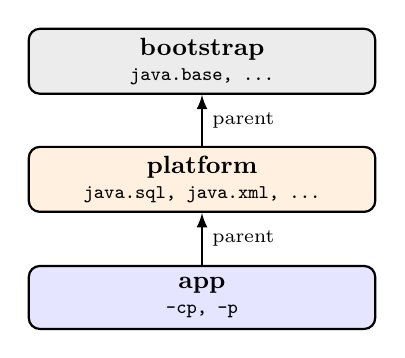
\begin{tikzpicture}[ld/.style={draw, rounded corners, thick, minimum width=4.4cm, minimum height=0.8cm, align=center, font=\small}]
        \node[ld, fill=gray!15] (b) at (0,0) {\textbf{bootstrap}\\[-2pt]{\scriptsize\ttfamily java.base, \dots}};
        \node[ld, fill=orange!12] (p) at (0,-1.5) {\textbf{platform}\\[-2pt]{\scriptsize\ttfamily java.sql, java.xml, \dots}};
        \node[ld, fill=blue!10] (a) at (0,-3) {\textbf{app}\\[-2pt]{\scriptsize\ttfamily -cp, -p}};
        \draw[-latex, thick] (a) -- node[right, font=\scriptsize] {parent} (p);
        \draw[-latex, thick] (p) -- node[right, font=\scriptsize] {parent} (b);
      \end{tikzpicture}
      \end{center}
    \end{column}
    \begin{column}{0.52\textwidth}
      \uncover<2->{\lstterminal[basicstyle=\ttfamily\scriptsize]{codeoutput/Loaders.txt}}
      \uncover<3->{
      \begin{itemize}\small
        \item A loader first asks its \textbf{parent}: a class path JAR cannot replace \texttt{java.lang.String}.
        \item The same name loaded by two loaders gives two \emph{different} classes (plugins, application servers).
      \end{itemize}}
    \end{column}
  \end{columns}
\end{frame}
% ~~~~~~~~~~~~~~~~~~~~~~~~~~~~~~~~~~~~~~ A frm




% ~~~~~~~~~~~~~~~~~~~~~~~~~~~~~~~~~~~~~~ V frm
\begin{frame}[t,fragile] \frametitle{Watching the JVM load classes: \texttt{-Xlog}}
  \lstterminal[basicstyle=\ttfamily\scriptsize]{codeoutput/ClassLoad.txt}

  \vspace{0.1em}
  \small
  About 550 classes are loaded to print one line; almost all come from the \textbf{CDS archive} (\emph{shared objects file}),
  a memory image of pre-parsed JDK classes. \texttt{-Xlog} is the unified logging of the JVM: \texttt{-Xlog:help} lists the tags
  (\texttt{gc}, \texttt{class+load}, \texttt{safepoint}, \dots).
\end{frame}
% ~~~~~~~~~~~~~~~~~~~~~~~~~~~~~~~~~~~~~~ A frm

% ~~~~~~~~~~~~~~~~~~~~~~~~~~~~~~~~~~~~~~ V
\hSection[Class files]{Class Files and Versions}{}{}
% ~~~~~~~~~~~~~~~~~~~~~~~~~~~~~~~~~~~~~~ A




% ~~~~~~~~~~~~~~~~~~~~~~~~~~~~~~~~~~~~~~ V frm
\begin{frame}[t,fragile] \frametitle{Inside a \texttt{.class} file}
  \begin{columns}[T]
    \begin{column}{0.44\textwidth}
      \begin{center}\small
      \begin{tabular}{rll}
        \toprule
        bytes & content & \\
        \midrule
        0--3  & magic             & \texttt{CA FE BA BE} \\
        4--5  & minor version     & \texttt{00 00} \\
        6--7  & major version     & \texttt{00 41} = 65 \\
        8--   & constant pool, \dots & \\
        \bottomrule
      \end{tabular}
      \end{center}
      \[
      	\mathit{major} = \mathit{release} + 44
      \]
      \small so Java 8 \(\to\) 52, 17 \(\to\) 61, 21 \(\to\) 65, 25 \(\to\) 69.
    \end{column}
    \begin{column}{0.54\textwidth}
      \lstterminal[basicstyle=\ttfamily\tiny]{codeoutput/Version.txt}
    \end{column}
  \end{columns}
  \vspace{0.2em}
  \small We changed byte 7 to \texttt{46} (= 70, Java 26): a JVM refuses class files \textbf{newer} than itself, but runs all older ones.
  Fix: run with a newer JDK, or compile with \texttt{--release 21}.
\end{frame}
% ~~~~~~~~~~~~~~~~~~~~~~~~~~~~~~~~~~~~~~ A frm

% ~~~~~~~~~~~~~~~~~~~~~~~~~~~~~~~~~~~~~~ V
\hSection[Start-up]{Start-up and Profiling}{}{}
% ~~~~~~~~~~~~~~~~~~~~~~~~~~~~~~~~~~~~~~ A

% ~~~~~~~~~~~~~~~~~~~~~~~~~~~~~~~~~~~~~~ V
\subsection[CDS]{Class data sharing}
% ~~~~~~~~~~~~~~~~~~~~~~~~~~~~~~~~~~~~~~ A




% ~~~~~~~~~~~~~~~~~~~~~~~~~~~~~~~~~~~~~~ V frm
\begin{frame}[t,fragile] \frametitle{Faster start-up with an application CDS archive}
  \lstterminal[basicstyle=\ttfamily\scriptsize]{codeoutput/Cds.txt}

  \vspace{0.1em}
  \small
  Five runs each (times differ from machine to machine). \texttt{-Xshare:off} disables the JDK's archive;
  \texttt{-XX:ArchiveClassesAtExit} (Java 13+) records the classes of one run, \texttt{-XX:SharedArchiveFile} maps them next time.
  Projects Leyden (Java 24+: \texttt{-XX:AOTCache}) and GraalVM \texttt{native-image} go further.
\end{frame}
% ~~~~~~~~~~~~~~~~~~~~~~~~~~~~~~~~~~~~~~ A frm

% ~~~~~~~~~~~~~~~~~~~~~~~~~~~~~~~~~~~~~~ V
\subsection[JFR]{Flight Recorder}
% ~~~~~~~~~~~~~~~~~~~~~~~~~~~~~~~~~~~~~~ A




% ~~~~~~~~~~~~~~~~~~~~~~~~~~~~~~~~~~~~~~ V frm
\begin{frame}[t,fragile] \frametitle{Profiling from the command line: JFR}
  \begin{columns}[T]
    \begin{column}{0.42\textwidth}
      \lstcode[basicstyle=\ttfamily\tiny]{codeoutput/Jfr/Work.java}{Java}
    \end{column}
    \begin{column}{0.56\textwidth}
      \uncover<2->{\lstterminal[basicstyle=\ttfamily\tiny]{codeoutput/Jfr.txt}}
    \end{column}
  \end{columns}

  \vspace{0.1em}
  \small The \textbf{JDK Flight Recorder} is built into the JVM with about 1\,\% overhead, so it can stay on in production.
  \texttt{jcmd <pid> JFR.start} attaches it to a running JVM; JDK Mission Control (a separate GUI) opens the \texttt{.jfr} file.
\end{frame}
% ~~~~~~~~~~~~~~~~~~~~~~~~~~~~~~~~~~~~~~ A frm

% ~~~~~~~~~~~~~~~~~~~~~~~~~~~~~~~~~~~~~~ V
\hSection[Security]{Trust and Supply Chain}{}{}
% ~~~~~~~~~~~~~~~~~~~~~~~~~~~~~~~~~~~~~~ A

% ~~~~~~~~~~~~~~~~~~~~~~~~~~~~~~~~~~~~~~ V
\subsection[Reproducible]{Reproducible builds}
% ~~~~~~~~~~~~~~~~~~~~~~~~~~~~~~~~~~~~~~ A




% ~~~~~~~~~~~~~~~~~~~~~~~~~~~~~~~~~~~~~~ V frm
\begin{frame}[t,fragile] \frametitle{Same sources, same JAR? \texttt{jar --date}}
  \lstterminal[basicstyle=\ttfamily\scriptsize]{codeoutput/Reproducible.txt}

  \vspace{0.1em}
  \small
  A JAR is a ZIP file that stores each entry's time, so two builds differ. \texttt{--date} (Java 19+) fixes all
  timestamps: anyone can rebuild and compare checksums. Maven: \texttt{project.build.outputTimestamp}.
\end{frame}
% ~~~~~~~~~~~~~~~~~~~~~~~~~~~~~~~~~~~~~~ A frm

% ~~~~~~~~~~~~~~~~~~~~~~~~~~~~~~~~~~~~~~ V
\subsection[Checksums]{Checksums}
% ~~~~~~~~~~~~~~~~~~~~~~~~~~~~~~~~~~~~~~ A




% ~~~~~~~~~~~~~~~~~~~~~~~~~~~~~~~~~~~~~~ V frm
\begin{frame}[t,fragile] \frametitle{Checking a download}
  \lstterminal[basicstyle=\ttfamily\scriptsize]{codeoutput/Checksum.txt}
  \vspace{0.2em}
  Every JDK download page publishes a SHA-256 checksum. Compare before installing:
  \begin{columns}[T]
    \begin{column}{0.48\textwidth}
      \begin{block}{Windows (Command Prompt)}


% +++++++++++++++++++++++++++++++++++++++ V lst
%: -Lst.
\begin{lstlisting}[style=codesnippet, language={}, basicstyle=\ttfamily\scriptsize]
certutil -hashfile OpenJDK21.msi SHA256
\end{lstlisting}
% +++++++++++++++++++++++++++++++++++++++ A lst


      \end{block}
    \end{column}
    \begin{column}{0.48\textwidth}
      \begin{block}{macOS (Terminal)}


% +++++++++++++++++++++++++++++++++++++++ V lst
%: -Lst.
\begin{lstlisting}[style=codesnippet, language=bash, basicstyle=\ttfamily\scriptsize]
shasum -a 256 OpenJDK21.pkg
\end{lstlisting}
% +++++++++++++++++++++++++++++++++++++++ A lst


      \end{block}
    \end{column}
  \end{columns}
\end{frame}
% ~~~~~~~~~~~~~~~~~~~~~~~~~~~~~~~~~~~~~~ A frm

% ~~~~~~~~~~~~~~~~~~~~~~~~~~~~~~~~~~~~~~ V
\subsection[Signing]{Signed JARs}
% ~~~~~~~~~~~~~~~~~~~~~~~~~~~~~~~~~~~~~~ A




% ~~~~~~~~~~~~~~~~~~~~~~~~~~~~~~~~~~~~~~ V frm
\begin{frame}[t,fragile] \frametitle{Signing and tampering}
  \lstterminal[basicstyle=\ttfamily\tiny]{codeoutput/Signing.txt}

  \vspace{0.1em}
  \small
  \texttt{jarsigner} stores a digest of every entry (\texttt{META-INF/*.SF}) and a signature (\texttt{*.RSA}).
  After we replaced \texttt{App.class}, verification and start-up both fail. Here the certificate is self-signed: real signing uses a
  certificate from a certificate authority. On \mac{} the \emph{installer} must also be signed and notarized (\texttt{jpackage --mac-sign}).
\end{frame}
% ~~~~~~~~~~~~~~~~~~~~~~~~~~~~~~~~~~~~~~ A frm




% ~~~~~~~~~~~~~~~~~~~~~~~~~~~~~~~~~~~~~~ V frm
\begin{frame}[t,fragile] \frametitle{Other risks on the command line}
  \begin{itemize}\small
    \item \textbf{Class path order}: a JAR placed \emph{before} yours can replace any of your classes; modules forbid split packages.
    \item \textbf{\texttt{CLASSPATH} and \texttt{JAVA\_TOOL\_OPTIONS}}: an attacker who can set the environment controls the JVM
      (\texttt{-javaagent:evil.jar}). Check them in CI logs: the JVM prints \emph{Picked up \dots}.
    \item \textbf{\texttt{PATH}}: which \texttt{java} runs? (\texttt{where java}, \texttt{which -a java})
    \item \textbf{Old JDKs}: only the latest update of an LTS gets security fixes (21.0.\emph{x}); update monthly or with each quarterly release.
    \item \textbf{Security Manager}: deprecated in Java 17 and permanently disabled in Java 24; isolate untrusted code with
      operating system processes or containers instead.
    \item \textbf{Secrets}: never on the command line (\texttt{-Dpassword=\dots} is visible in \texttt{ps} and \texttt{jcmd VM.command\_line}).
  \end{itemize}
\end{frame}
% ~~~~~~~~~~~~~~~~~~~~~~~~~~~~~~~~~~~~~~ A frm

% ~~~~~~~~~~~~~~~~~~~~~~~~~~~~~~~~~~~~~~ V
\hSection[Delivery]{Delivery Beyond the Laptop}{}{}
% ~~~~~~~~~~~~~~~~~~~~~~~~~~~~~~~~~~~~~~ A




% ~~~~~~~~~~~~~~~~~~~~~~~~~~~~~~~~~~~~~~ V frm
\begin{frame}[t,fragile] \frametitle{A container image with a jlink runtime}
  \begin{columns}[T]
    \begin{column}{0.6\textwidth}


% +++++++++++++++++++++++++++++++++++++++ V lst
%: -Lst.
\begin{lstlisting}[style=codesnippet, language=bash, basicstyle=\ttfamily\tiny]
# ---- stage 1: build with a full JDK
FROM eclipse-temurin:21-jdk AS build
WORKDIR /src
COPY src src
RUN javac -d mods --module-source-path src -m com.greet,com.app \
 && jlink -p mods --add-modules com.app --strip-debug \
          --no-header-files --no-man-pages --output /rt

# ---- stage 2: only the runtime and the application
FROM debian:bookworm-slim
COPY --from=build /rt /opt/app
USER 1000
ENTRYPOINT ["/opt/app/bin/java", "-m", "com.app/com.app.Main"]
\end{lstlisting}
% +++++++++++++++++++++++++++++++++++++++ A lst


    \end{column}
    \begin{column}{0.38\textwidth}
      \small


% +++++++++++++++++++++++++++++++++++++++ V lst
%: -Lst.
\begin{lstlisting}[style=codesnippet, language=bash, basicstyle=\ttfamily\scriptsize]
docker build -t hello .
docker run --rm hello
\end{lstlisting}
% +++++++++++++++++++++++++++++++++++++++ A lst


      Same commands on \win{} and \mac{} with Docker Desktop.
      The JVM sees the container's CPU and memory limits; tune with \texttt{-XX:MaxRAMPercentage=75}.
      \hRemark{Not run here.}
    \end{column}
  \end{columns}
\end{frame}
% ~~~~~~~~~~~~~~~~~~~~~~~~~~~~~~~~~~~~~~ A frm




% ~~~~~~~~~~~~~~~~~~~~~~~~~~~~~~~~~~~~~~ V frm
\begin{frame}[t,fragile] \frametitle{Native executables: GraalVM \texttt{native-image}}
  \begin{columns}[T]
    \begin{column}{0.48\textwidth}


% +++++++++++++++++++++++++++++++++++++++ V lst
%: -Lst.
\begin{lstlisting}[style=codesnippet, language=bash, basicstyle=\ttfamily\scriptsize]
javac -d out App.java
native-image -cp out App app
./app            # starts in milliseconds
\end{lstlisting}
% +++++++++++++++++++++++++++++++++++++++ A lst


      \small \hRemark{Not run here} (needs GraalVM). On \win{} it needs the Visual Studio C++ build tools and makes \texttt{app.exe};
      on \mac{} the Xcode command line tools.
    \end{column}
    \begin{column}{0.48\textwidth}
      \begin{center}\scriptsize
      \begin{tabular}{lcc}
        \toprule
                          & JVM               & native image \\
        \midrule
        start-up          & 50--500 ms        & 1--50 ms \\
        peak speed        & JIT, very high    & good \\
        build time        & seconds           & minutes \\
        reflection        & free              & must be declared \\
        one binary for    & every OS          & one OS + CPU \\
        \bottomrule
      \end{tabular}
      \end{center}
    \end{column}
  \end{columns}
\end{frame}
% ~~~~~~~~~~~~~~~~~~~~~~~~~~~~~~~~~~~~~~ A frm

% ~~~~~~~~~~~~~~~~~~~~~~~~~~~~~~~~~~~~~~ V
\hSection[Debugging]{Remote Debugging and Diagnostics}{}{}
% ~~~~~~~~~~~~~~~~~~~~~~~~~~~~~~~~~~~~~~ A




% ~~~~~~~~~~~~~~~~~~~~~~~~~~~~~~~~~~~~~~ V frm
\begin{frame}[t,fragile] \frametitle{Diagnostics without an IDE}
  \begin{center}\tiny
  \begin{tabular}{ll}
    \toprule
    need                         & command \\
    \midrule
    wait for a debugger          & \texttt{java -agentlib:jdwp=transport=dt\_socket,server=y,suspend=y,address=*:5005 -jar app.jar} \\
    debug in the terminal        & \texttt{jdb -attach 5005} (or attach an IDE to port 5005) \\
    thread dump                  & \texttt{jcmd <pid> Thread.print}; macOS/Linux also \texttt{kill -3 <pid>}; \win{} \texttt{Ctrl+Break} \\
    heap dump                    & \texttt{jcmd <pid> GC.heap\_dump heap.hprof} \\
    dump on crash                & \texttt{-XX:+HeapDumpOnOutOfMemoryError -XX:HeapDumpPath=dumps} \\
    garbage collector log        & \texttt{-Xlog:gc*:file=gc.log:time,uptime} \\
    record a profile             & \texttt{-XX:StartFlightRecording=duration=60s,filename=r.jfr} \\
    JVM settings of a process    & \texttt{jcmd <pid> VM.flags}, \texttt{VM.system\_properties}, \texttt{VM.command\_line} \\
    \bottomrule
  \end{tabular}
  \end{center}
  \small \texttt{address=*:5005} opens a port to the network: on a server use \texttt{localhost:5005} and an SSH tunnel.
\end{frame}
% ~~~~~~~~~~~~~~~~~~~~~~~~~~~~~~~~~~~~~~ A frm

% ~~~~~~~~~~~~~~~~~~~~~~~~~~~~~~~~~~~~~~ V
\hSection[Summary]{Summary}{}{}
% ~~~~~~~~~~~~~~~~~~~~~~~~~~~~~~~~~~~~~~ A




% ~~~~~~~~~~~~~~~~~~~~~~~~~~~~~~~~~~~~~~ V frm
\begin{frame}[t,fragile] \frametitle{Big ideas}
  \begin{itemize}
    \item The \texttt{java} command is a small native launcher; options can come from the command line, \texttt{@files},
      \texttt{JDK\_JAVA\_OPTIONS} and \texttt{JAVA\_TOOL\_OPTIONS}.
    \item Classes are loaded on demand by three loaders; CDS archives make start-up fast.
    \item A class file carries its version: newer class files do not run on older JVMs.
    \item Builds should be \textbf{reproducible}, downloads \textbf{checked}, artifacts \textbf{signed}.
    \item Delivery options grow from JAR to \texttt{jlink} image, installer, container and native executable;
      each one trades size, start-up and portability.
    \item The JDK's own tools (\texttt{jcmd}, \texttt{jfr}, \texttt{jdb}, \texttt{-Xlog}) diagnose a JVM anywhere a terminal exists.
  \end{itemize}
\end{frame}
% ~~~~~~~~~~~~~~~~~~~~~~~~~~~~~~~~~~~~~~ A frm




% ~~~~~~~~~~~~~~~~~~~~~~~~~~~~~~~~~~~~~~ V frm
\begin{frame}[t,fragile] \frametitle{Projects}
  \begin{enumerate}\small
    \item Write \texttt{build.sh} and \texttt{build.bat} that build the books application reproducibly; prove it with two
      checksums on two different computers (one Windows, one macOS).
    \item Measure start-up of the books application as a JAR, with AppCDS, as a \texttt{jlink} image and (optionally) as a
      native image. Report median times of 20 runs.
    \item Sign the JAR, change one byte, and explain every line printed by \texttt{jarsigner -verify -verbose}.
    \item Record a JFR file of \texttt{Work}, find the hottest method with \texttt{jfr print}, make it faster, record again.
    \item Write a launcher script that picks the newest installed JDK $\geq 21$ on Windows (\texttt{where}) and macOS
      (\texttt{java\_home}) and prints a clear message if none exists.
  \end{enumerate}
\end{frame}
% ~~~~~~~~~~~~~~~~~~~~~~~~~~~~~~~~~~~~~~ A frm




% ~~~~~~~~~~~~~~~~~~~~~~~~~~~~~~~~~~~~~~ V frm
\begin{frame}[t,fragile]
	\begin{center}
		\vspace{4cm}
		\hRemark{\Huge Questions?}
	\end{center}
\end{frame}
% ~~~~~~~~~~~~~~~~~~~~~~~~~~~~~~~~~~~~~~ A frm



\end{document}
